\clearpage
\section*{Practice A: Populations and samples}
These are the chapter's original practice situations. Name the group of interest before discussing what the selection method may miss.
\begin{enumerate}[label=A\arabic*.,leftmargin=2.5em,itemsep=10pt]
\item For each situation, identify the population and sample. Explain which parts of the population the sampling method might overrepresent or underrepresent.
\begin{enumerate}[label=(\alph*)]
\item A hospital uses ER patients from last Tuesday to estimate the average wait time for the whole month.
\item A polling organization calls 1,000 randomly selected registered voters to estimate support for a ballot measure.
\item A coffee shop asks only Monday-morning customers whether the shop should open earlier.
\end{enumerate}
\item A researcher wants to estimate daily screen time for teenagers in a city. Describe a simple random sampling plan, assuming a complete list is available. Describe a plan that would systematically favor part of the population.
\item Explain in two sentences why a larger sample does not automatically correct a problem in how the sample is selected.
\end{enumerate}

\Needspace{8\baselineskip}
\section*{Practice B: Frequency tables}
\begin{enumerate}[label=B\arabic*.,leftmargin=2.5em,itemsep=10pt]
\item The sibling counts reported by 18 students are
\[2,0,1,3,1,2,0,1,1,2,3,0,1,2,1,0,2,1.\]
Construct a frequency table, identify a most common number of siblings, and verify the total count.
\item Twenty employees report these usual travel methods:
\begin{quote}car, bus, car, bike, car, walk, car, bus, bike, car, car, walk, bus, car, bike, car, bus, car, walk, car.\end{quote}
Construct a frequency table. Which method is most common? How many employees use something other than a car?
\item The first three categories in a four-category table have frequencies 8, 12, and 5. The sample has 30 observations. Find the fourth frequency.
\end{enumerate}

\Needspace{8\baselineskip}
\section*{Practice C: Relative frequency and probability}
\begin{enumerate}[label=C\arabic*.,leftmargin=2.5em,itemsep=10pt]
\item Use the sibling data in B1. Give each relative frequency as a fraction and decimal, and check their total. Find the probability of exactly one sibling when choosing uniformly from these 18 students. Find the probability of more than one sibling in the same group.
\item A fair spinner has five equal sections: red, orange, yellow, green, blue. Find the probability of each color, of not red, and of red or orange.
\item Roll one fair six-sided die. Construct its probability distribution. Find P(4), P(even), and P(greater than 4).
\item A four-outcome distribution has probabilities 0.15, 0.30, 0.25, and p. Find p and explain the rule you use.
\end{enumerate}

\Needspace{8\baselineskip}
\section*{Practice D: Bar charts}
\begin{enumerate}[label=D\arabic*.,leftmargin=2.5em,itemsep=10pt]
\item Use the employee transportation data in B2. Compute each relative frequency and draw a labeled bar chart. Name a pair of methods whose combined share is more than half of the commuters. Is there more than one valid pair?
\item Use the book-club chart below. How many members are represented? What share read exactly one book? What is the probability that a randomly selected member read more than two books?
\begin{center}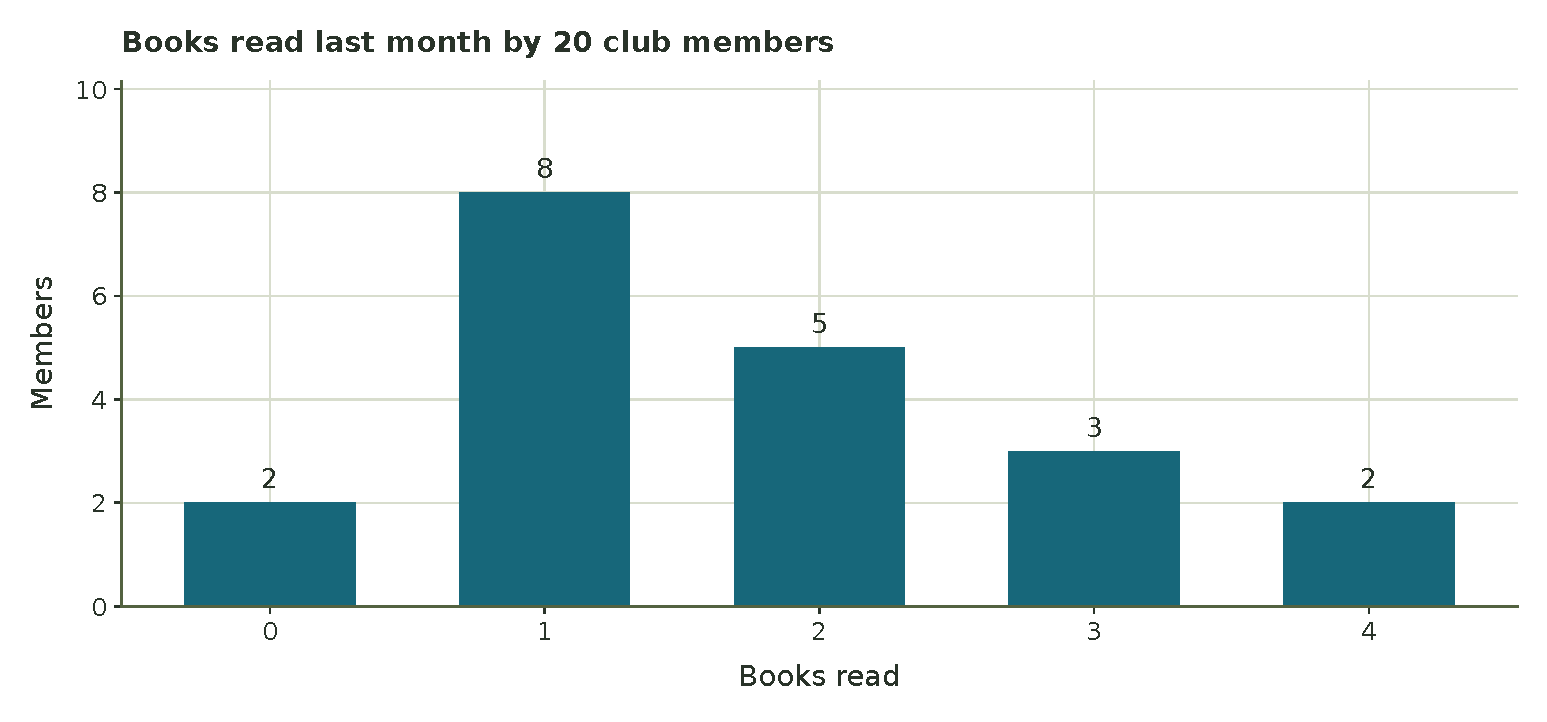
\includegraphics[width=\linewidth,height=2.6in,keepaspectratio]{../assets/week2/book-club.pdf}\end{center}
\item Forty office workers report their preferred lunch location: cafeteria 18, restaurant 10, desk 8, outside 4. Draw a bar chart of relative frequencies and identify the most and least common preferences.
\end{enumerate}

\Needspace{8\baselineskip}
\section*{Practice E: Histograms}
Use the stated left-closed, right-open bins: [a,b) includes a and excludes b.
\begin{enumerate}[label=E\arabic*.,leftmargin=2.5em,itemsep=10pt]
\item The ages of 24 volunteers are
\begin{quote}22, 25, 31, 28, 35, 22, 29, 40, 33, 27, 25, 38, 30, 26, 42, 23, 31, 29, 35, 24, 27, 33, 28, 36.\end{quote}
Group the ages into [20,25), [25,30), [30,35), [35,40), [40,45). Construct a frequency table, draw a relative-frequency histogram, and identify the bin with the greatest count.
\item Use the weekly social-media-hours histogram below. How many students are represented? What is the relative frequency of [10,15) hours? Describe its shape and justify your answer.
\begin{center}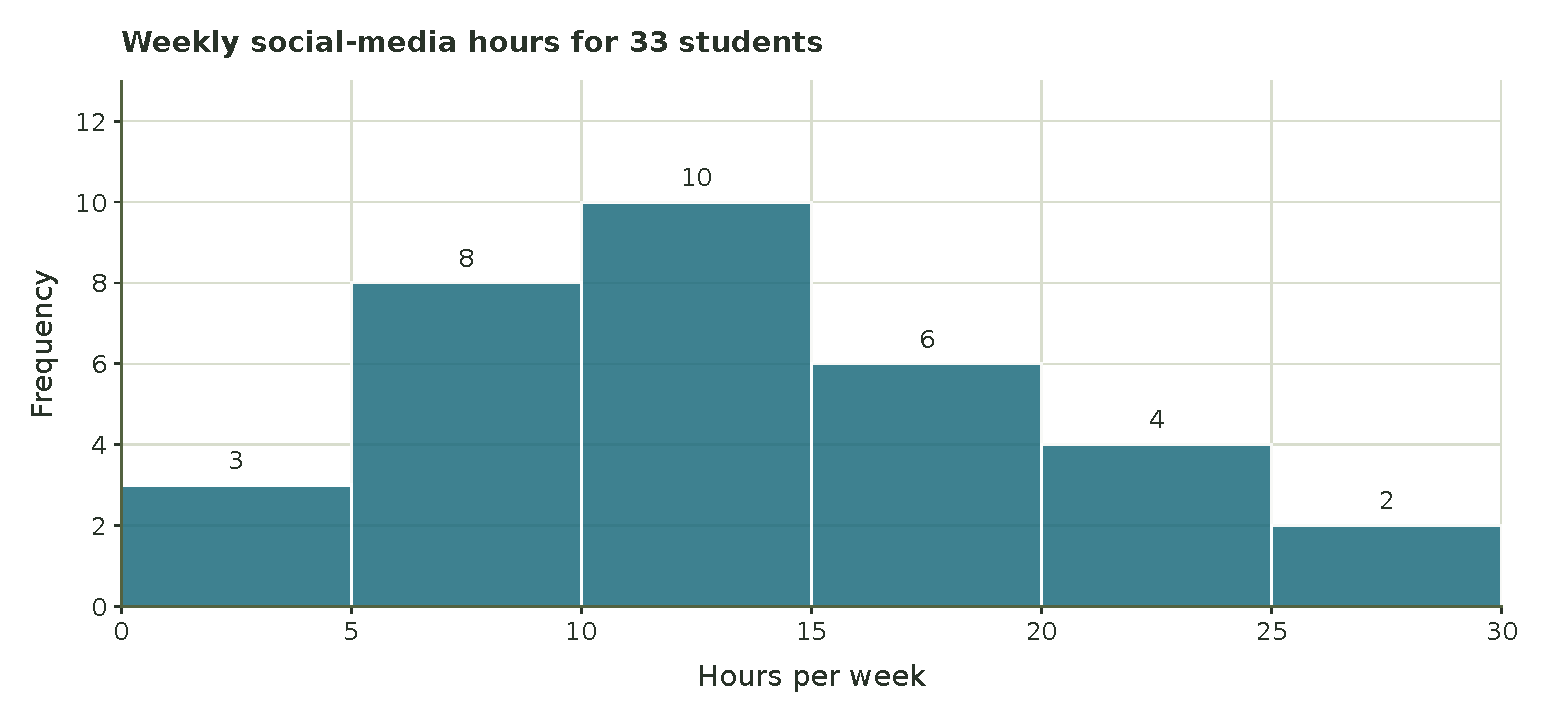
\includegraphics[width=\linewidth,height=2.7in,keepaspectratio]{../assets/week2/social-hours.pdf}\end{center}
\item Explain the difference between a bar chart and a histogram. Give one appropriate example for each.
\end{enumerate}

\Needspace{8\baselineskip}
\section*{Practice F: Probability distributions}
\begin{enumerate}[label=F\arabic*.,leftmargin=2.5em,itemsep=10pt]
\item Decide whether each complete list is a valid probability distribution. Explain any failure.
\begin{enumerate}[label=(\alph*)]
\item A, B, C with probabilities 0.3, 0.5, 0.2.
\item A, B, C with probabilities 0.4, 0.4, 0.4.
\item A, B with probabilities 0.7 and $-0.3$.
\item A, B, C, D with probabilities 0.25 each.
\end{enumerate}
\item A bag has 3 red, 4 blue, and 5 green chips. Each chip is equally likely to be drawn. Construct the color distribution, draw a bar chart, and find P(not blue).
\item For two fair independent six-sided dice, find P(sum $\leq6$) and P(sum $\geq8$). Explain why they are equal.
\item The number of errors in a randomly selected document has the distribution below.
\begin{center}\begin{tabular}{lrrrrr}\toprule
Errors & 0 & 1 & 2 & 3 & 4\\
Probability & .50 & .30 & .12 & .05 & .03\\\bottomrule
\end{tabular}\end{center}
Verify the distribution. Find P(at least one error). Sketch its numerical probability display using equal-width bars centered at the integer error counts. Describe its shape.
\end{enumerate}

\Needspace{8\baselineskip}
\section*{Chapter 2 Review}
\begin{enumerate}[label=R\arabic*.,leftmargin=2.5em,itemsep=10pt]
\item A team inspects 50 products: 0 defects for 28 items, 1 defect for 14, 2 defects for 6, and 3 defects for 2. Construct frequency and relative-frequency tables. Draw a histogram with width-one bins centered at the integer defect counts. Find the probability that a uniformly chosen inspected item has at least one defect. Describe the shape.
\item Sixty commuters have recorded travel times: [0,15) minutes, 12 commuters; [15,30), 22; [30,45), 18; [45,60), 8. Construct a relative-frequency table and histogram. Find the share with travel time at least 15 and less than 45 minutes.
\item A spinner's first three section probabilities are $1/3$, $1/4$, and $1/6$. Find the fourth probability p. Find the probability of one of the first two sections.
\item Explain in two sentences the difference between empirical and theoretical probability distributions, giving an example of each.
\item Thirty students report last night's sleep: 4 hours for 2 students, 5 for 4, 6 for 8, 7 for 10, 8 for 5, and 9 for 1. Construct a relative-frequency table and histogram with width-one bins centered at the reported hours. Describe the shape, a rough center, and the observed spread. Find the probability that a uniformly chosen student from this group slept fewer than 7 hours.
\item An administrator uses one advisory class to describe a school of 400 students, with 100 in each of four grade levels. The advisory has 20 students, all seniors. Identify population and sample. Explain in two sentences what the selection leaves out.
\end{enumerate}
